<\chapter{Dsm}
In questo capitolo verrà riportato dettagliatamente il funzionamento e la strutturazione del componente dsm necessario alla comunicazione tra agenti, nello specifico verra spiegato come è stato realizzato il tuple space e tutti i meccanismi ad esso correlati.
Per il progetto in questione sono stati realizzati i comandi prettamente necessari, che sono: IN, OUT, UPDATE e READ \cite{linda}.
\section{DsmData}
Per la gestione dei dati è stato realizzato una sorta di database volatile tramite lo sfruttamento di \var{Hashtable} e \var{Queue}. In particolare si realizzata una struttura del genere:
\begin{figure}[H]
\begin{center}
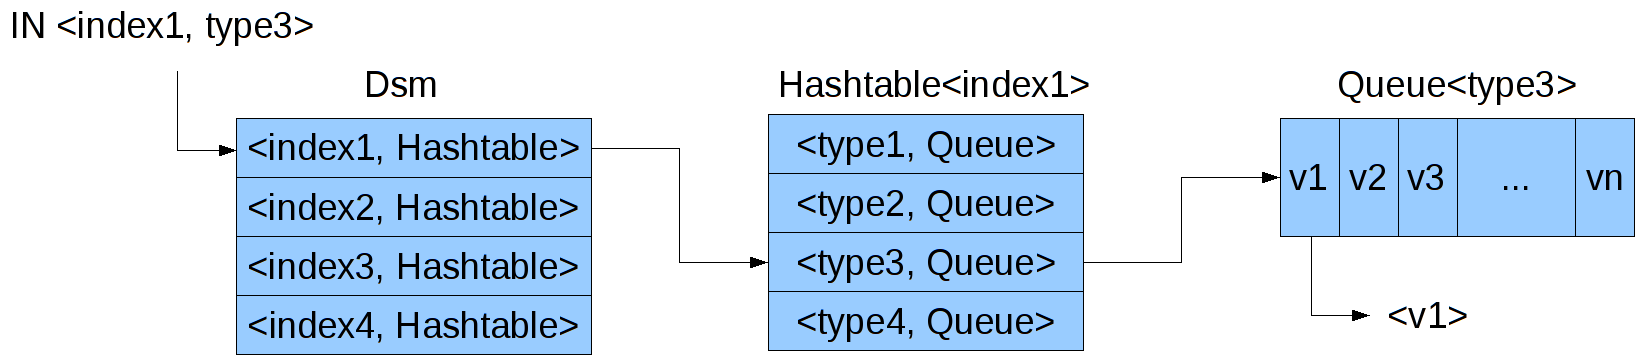
\includegraphics[scale=0.3]{etc/dsm.png}
\caption{Esempio di IN nel Dsm}
\label{dsm1}
\end{center}
\end{figure}
Dalla figura è riportato un esempio delle operazioni eseguite sul database nel momento in cui si effettua una richiesta \code{IN <index1, type3>}, ovvero si richiede un valore di tipo 3 che si trova nell'indice 1. Le operazioni eseguite sono elencate di seguito:
\begin{enumerate}
	\item Quando perviene la richiesta al db si cerca immediatamente la presenza di una chiave \code{index1} nell'hashtable di primo livello;
	\item se la chiave è presente si prende l'hashtable associata e si procede con il controllo delle presenza della chiave \code{type3} all'interno dell'hashtable di secondo livello;
	\item se la chiave è presente si prende la coda che gli è associata e si estrae il valore che si trova in testa.
\end{enumerate}
Operazioni analoghe vengono effettuate per gli altri tipi di operazioni; in particolare le operazioni implementate hanno il seguente comportamento:
\begin{description}
	\item[OUT:] equivale alla tupla \code{OUT <index1, type3, v1>} e consiste nell'inserire un valore sul tuple space.
	\item[IN:] è rappresentata dalla tupla \code{IN <index1, type3>} ed il suo scopo è reperire il valore in testa alla coda e quindi eliminarlo dal tuple space.
	\item[READ:] tupla uguale a IN, ma ha l'unica differenza di non eliminare il valore dopo averlo reperito.
	\item[UPDATE:] tupla come OUT con la differenza che se il valore esiste lo sostituisce.
\end{description}
\section{DsmClient}
Questo componente consente la comunicazione con il server dsm sfruttando lo scambio di messaggi che mette a disposizione Jade con il suo \var{framework}. Il modulo in questione consente due meccanismi principali che sono: l'invio di messaggi bloccanti e l'invio di messaggi non bloccanti. Per quanto riguarda i messaggi bloccanti (IN e READ) si ha:
\begin{enumerate}
	\item Il Client invia la richiesta al server ed attende la risposta;
	\item Il Server riceve la richiesta, la esaurisce ed invia la risposta;
	\item Il Client riceve la richiesta e la ritorna all'agente chiamante.
\end{enumerate}
I messaggi non bloccanti di tipo OUT e UPDATE, invece, vengono inviati nel seguente modo:
\begin{enumerate}
	\item Il Client invia la richiesta al server e ritorna all'agente chiamante;
	\item Il Server riceve la richiesta e la esaurisce;
\end{enumerate}
\section{DsmServer}
Tale componente può essere inteso come un \var{proxy} in quanto non fa altro che tradurre le richieste del client a operazioni sul \code{DsmData} e quindi ritornare una risposta (in caso di messaggi bloccanti). Una caratteristica importante di questo agente è che può migrare tra i vari nodi in base alla disponibilità delle risorse dei nodi, nello specifico non fa altro che seguire lo \var{SC}, ovvero quando lo SC migra su un altro nodo il DsmServer lo segue (rif SC).